\section{Szyfrowanie}

\begin{frame}
	\begin{alertblock}{Szyfrowanie}
		Jest to proces przetwarzania przesyłanej informacji w taki sposób, by była czytelna tylko dla uprawnionych stron komunikacji. Wiadomość zostaje przesłana w zakodowanej postaci, co znacznie utrudnia lub uniemożliwia zrozumienie jej treści w przypadku przechwycenia.
	\end{alertblock}
\end{frame}

\begin{frame}{Z kluczem prywatnym}
	Zarówno odbiorca, jak i nadawca dysponują takim samym kluczem.\\
	\vspace{\fill}
	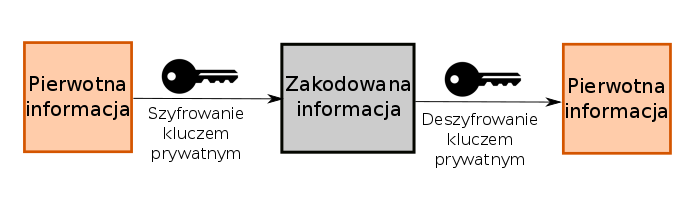
\includegraphics[height=0.25\paperwidth]{images/priv-key.png}
	\vspace{\fill}
	Obie strony muszą znać klucz przed rozpoczęciem komunikacji. Zwiększa to prawdopodobieństwo jego przechwycenia.	
\end{frame}

\begin{frame}{Z kluczem publicznym}
		\begin{itemize}
			\item Generowane są dwa klucze, prywatny i publiczny.
			\item Klucz publiczny jest ogólnie dostępny.
			\item Utworzenie dwóch takich par eliminuje konieczność wymiany kluczów prywatnych. 
		\end{itemize}	
\end{frame}

\begin{frame}{Z kluczem publicznym}
		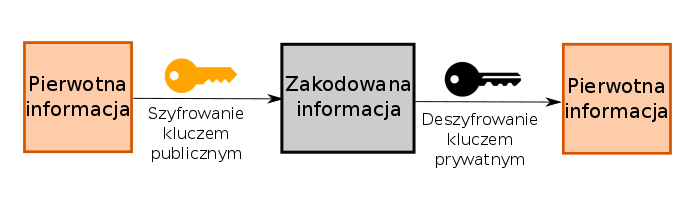
\includegraphics[height=0.25\paperwidth]{images/pub-key.png} \\
		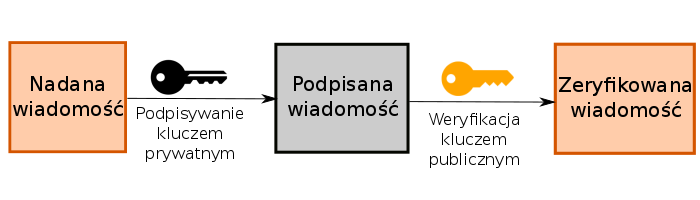
\includegraphics[height=0.25\paperwidth]{images/pub-key-sign.png}
\end{frame}

\begin{frame}{Algorytmy szyfrujące}
	\begin{itemize}
		\item Digital Signature Algorithm (DSA).
		\item ElGamal.
		\item NTRUEncrypt.
		\item Algorytmy bazujące na kryptografii krzywych eliptycznych.
		\item RSA.
	\end{itemize}
\end{frame}

\subsection{Protokoły}

\begin{frame}{IPsec}
	
\end{frame}

\begin{frame}{SSH}
	
\end{frame}

\begin{frame}{SSL}
	
\end{frame}

\begin{frame}{TSL}
	
\end{frame}

\begin{frame}{HTTPS, SFTP, FTPS}
	
\end{frame}

